\section{Szczegółowa analiza najlepszych modeli}

\subsection{SimpleMLP}

\begin{figure}[H]
\centering
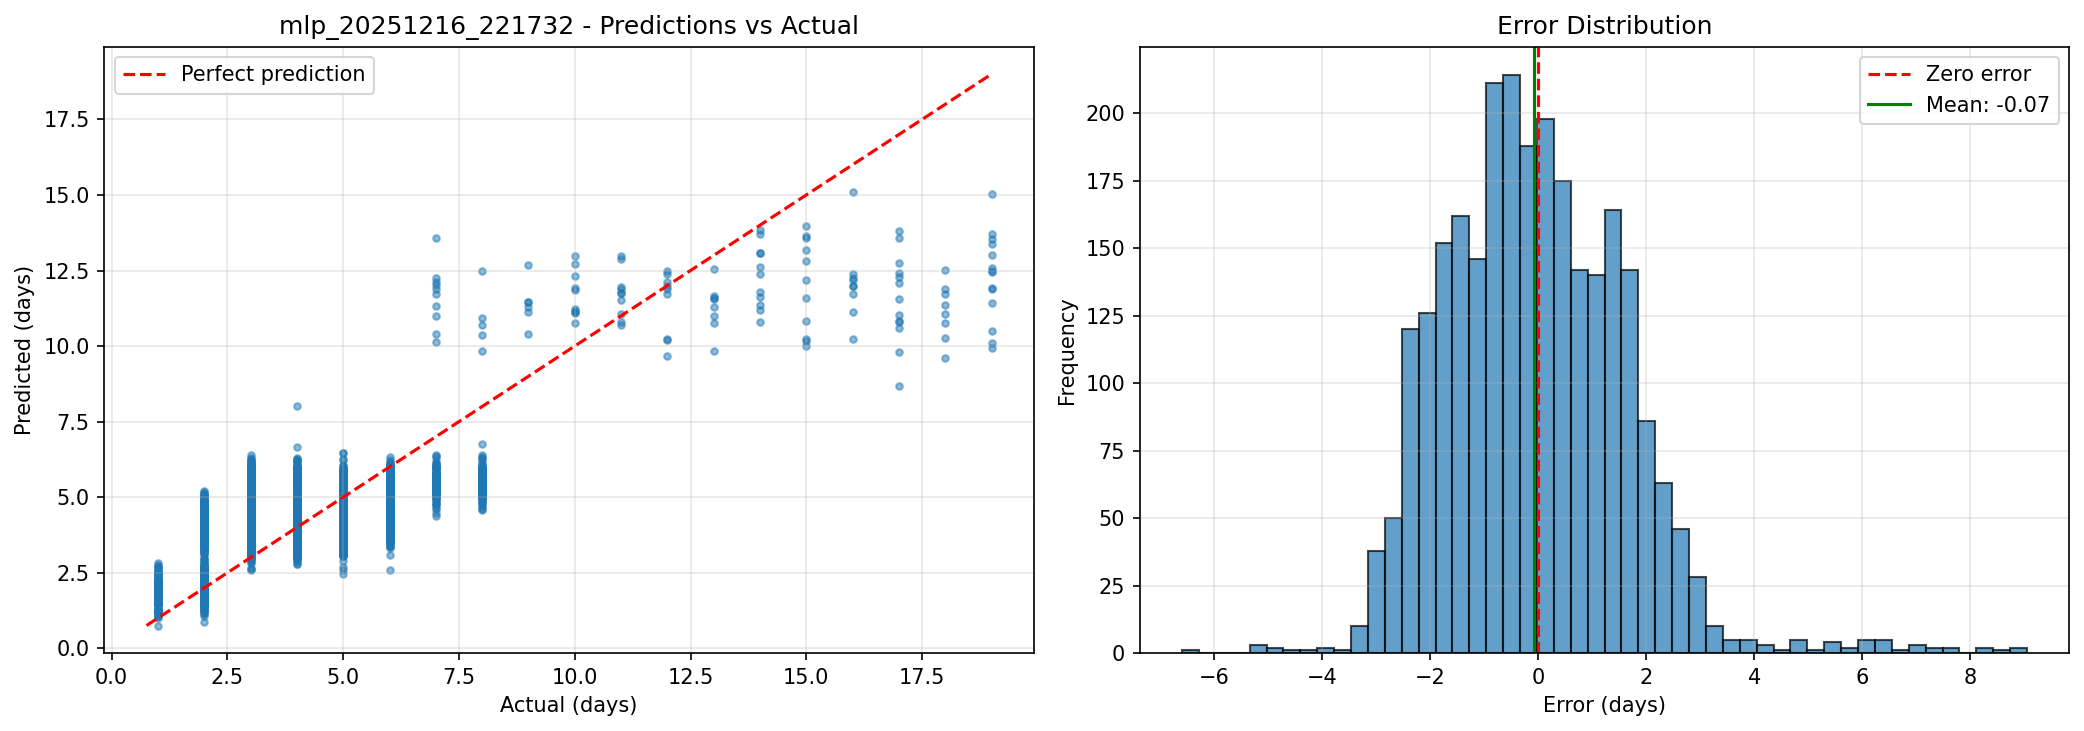
\includegraphics[width=0.45\textwidth]{figures/mlp_predictions.pdf}
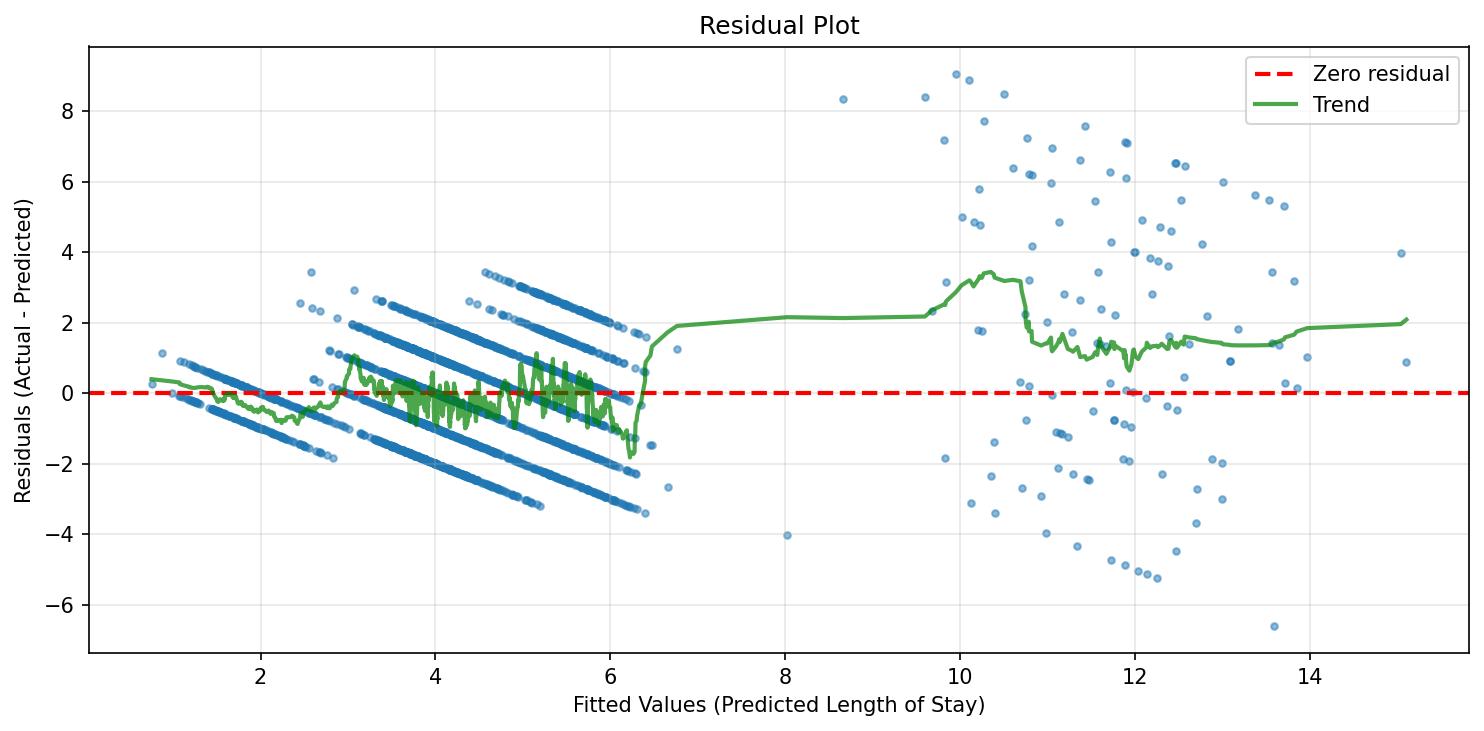
\includegraphics[width=0.45\textwidth]{figures/mlp_residuals.pdf}
\caption{Predykcje i reszty dla SimpleMLP}
\end{figure}

Model wykazał dobr ą korelację między predykcjami a wartościami rzeczywistymi. Reszty są losowo rozłożone z tendencją do większych błędów dla długich pobytów.

\subsection{TabNet}

\begin{figure}[H]
\centering
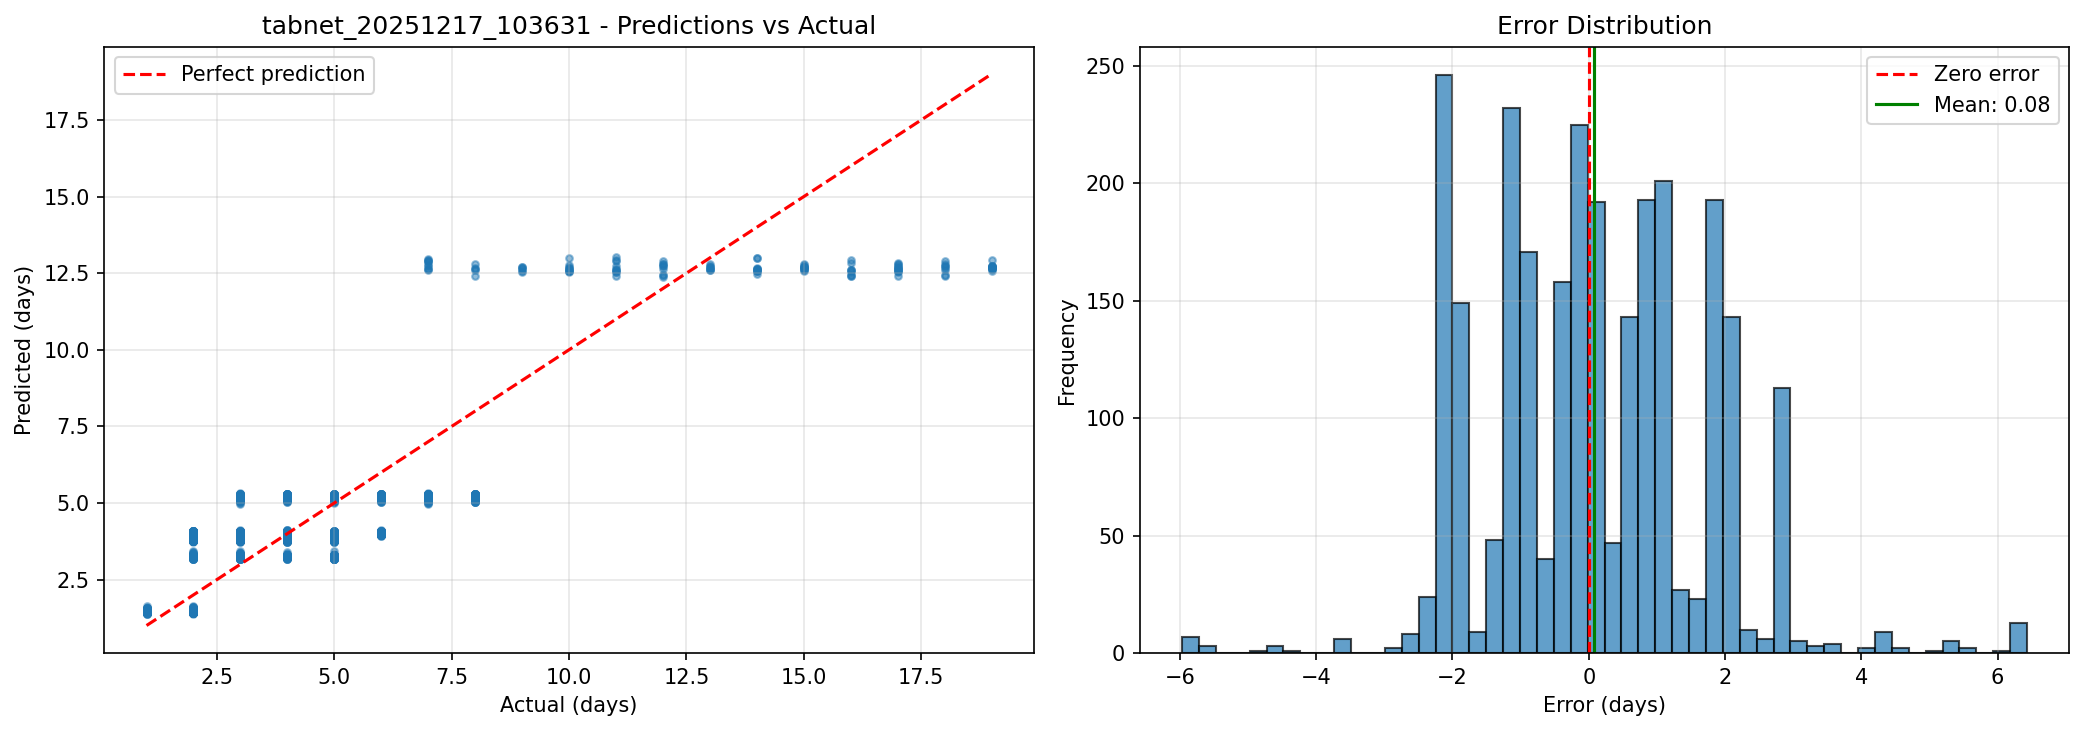
\includegraphics[width=0.45\textwidth]{figures/tabnet_predictions.pdf}
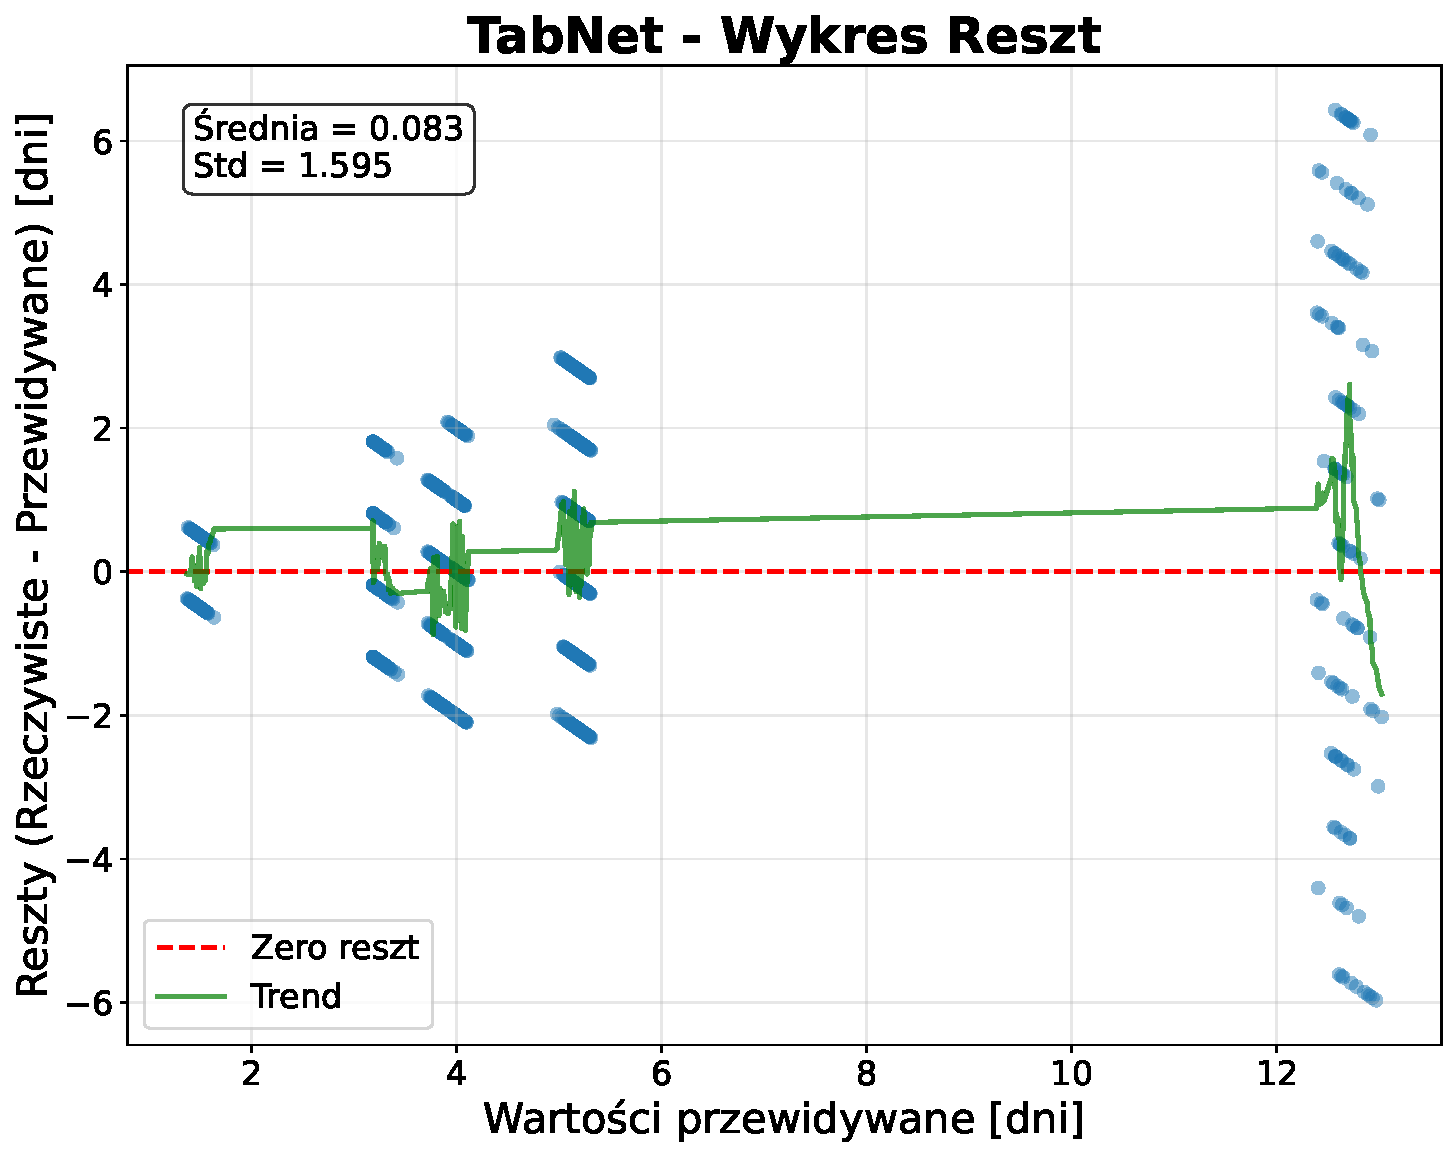
\includegraphics[width=0.45\textwidth]{figures/tabnet_residuals.pdf}
\caption{Predykcje i reszty dla TabNet}
\end{figure}

Najlepsze dopasowanie ze wszystkich modeli. Równomierne rozproszenie reszt wskazuje na homoskedastyczność. Mechanizm attention pozwala na interpretację decyzji modelu.

\subsection{TabTransformer}

\begin{figure}[H]
\centering
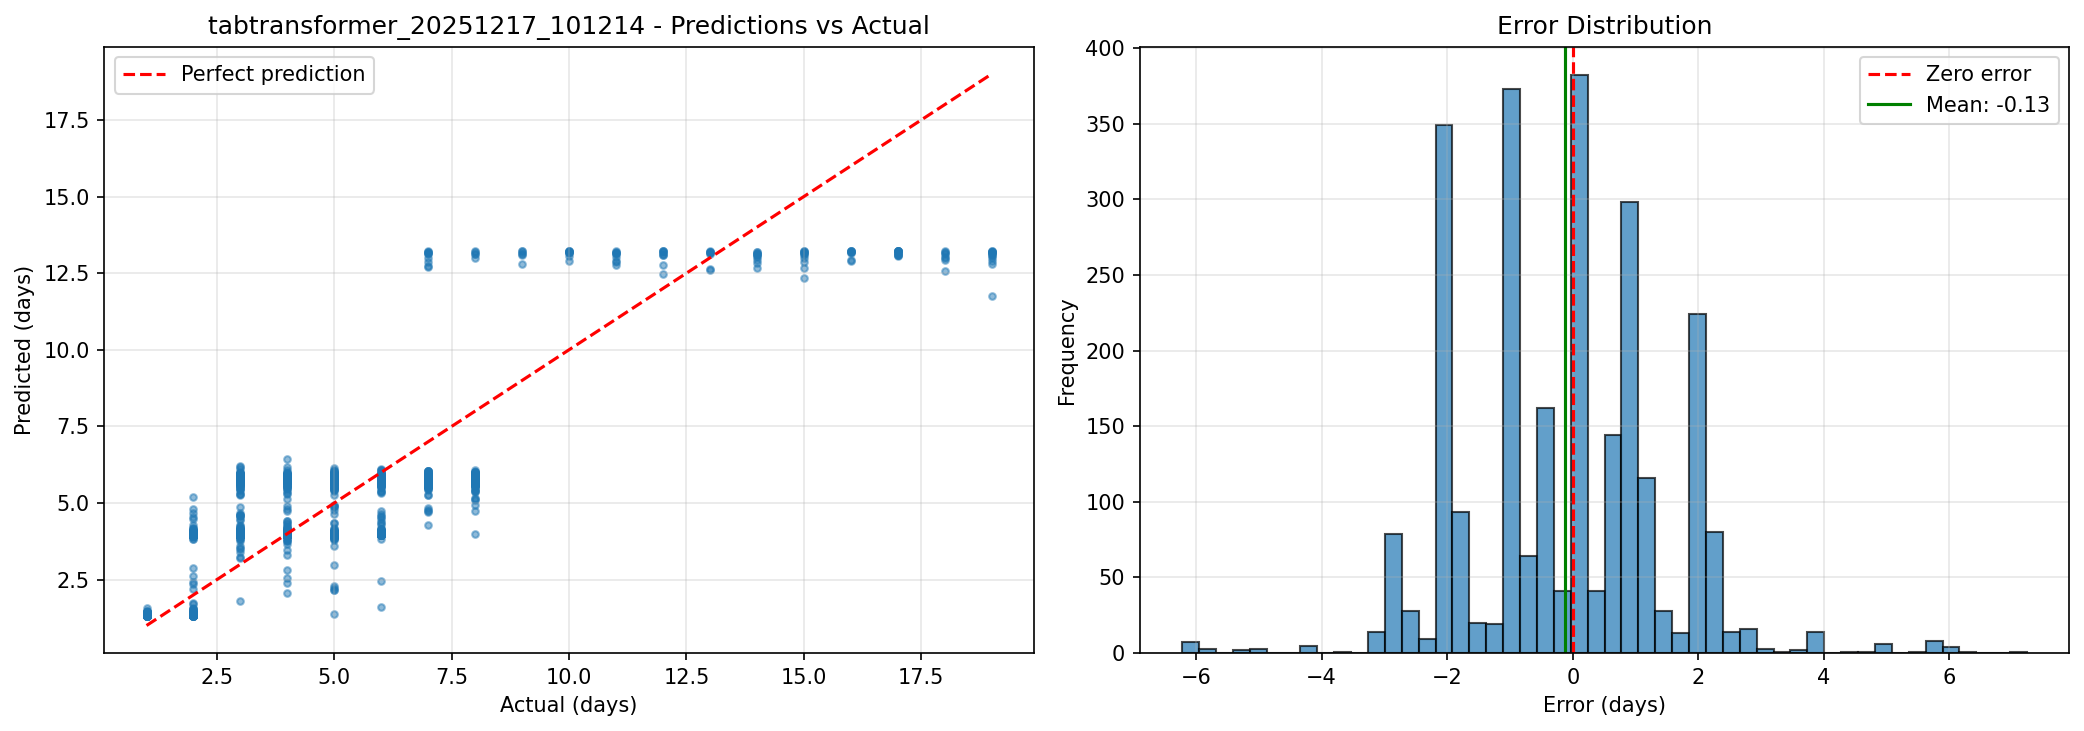
\includegraphics[width=0.45\textwidth]{figures/tabtransformer_predictions.pdf}
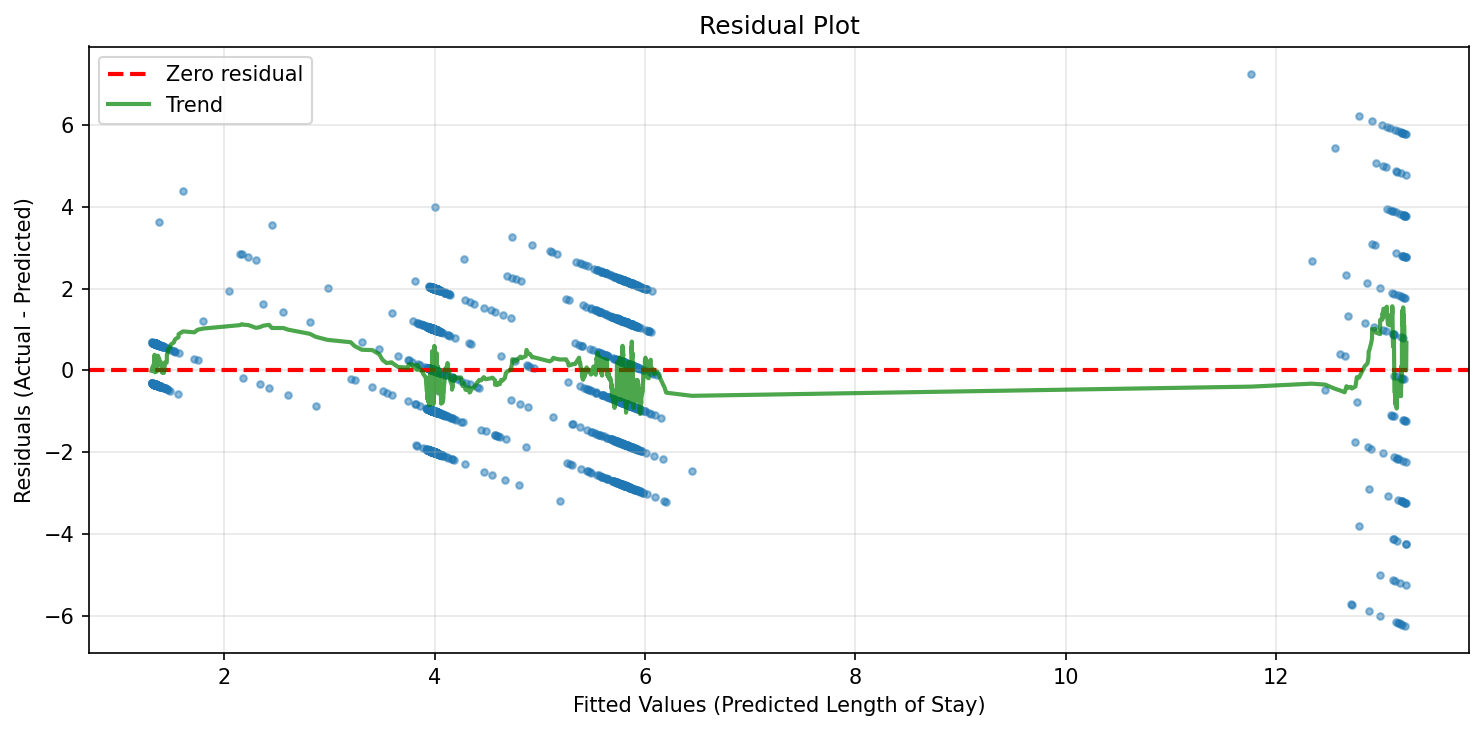
\includegraphics[width=0.45\textwidth]{figures/tabtransformer_residuals.pdf}
\caption{Predykcje i reszty dla TabTransformer}
\end{figure}

Bardzo dobre dopasowanie, porównywalne z TabNet. Stabilna wariancja reszt w całym zakresie wartości.
